\begin{frame}{$K^0$ $\cos\theta_{K0}$ vs $mom_{K_0}$ (Background)}
  \begin{tabular}{cc}
    \begin{minipage}{0.5\hsize}
      \centering
      Each background dist.
      \tiny
      \tminipageTwo{
        \begin{figure}
          $K^-d \rightarrow \pi^- "\Sigma^+" n_{detected}$
          \includegraphics[width=2.7cm]{../pic/Run78/QE/K0_cos_mom_pimSp.eps}
        \end{figure}
      }{
        \begin{figure}
          $K^-d \rightarrow \pi^+ "\Sigma^-" n_{detected}$
          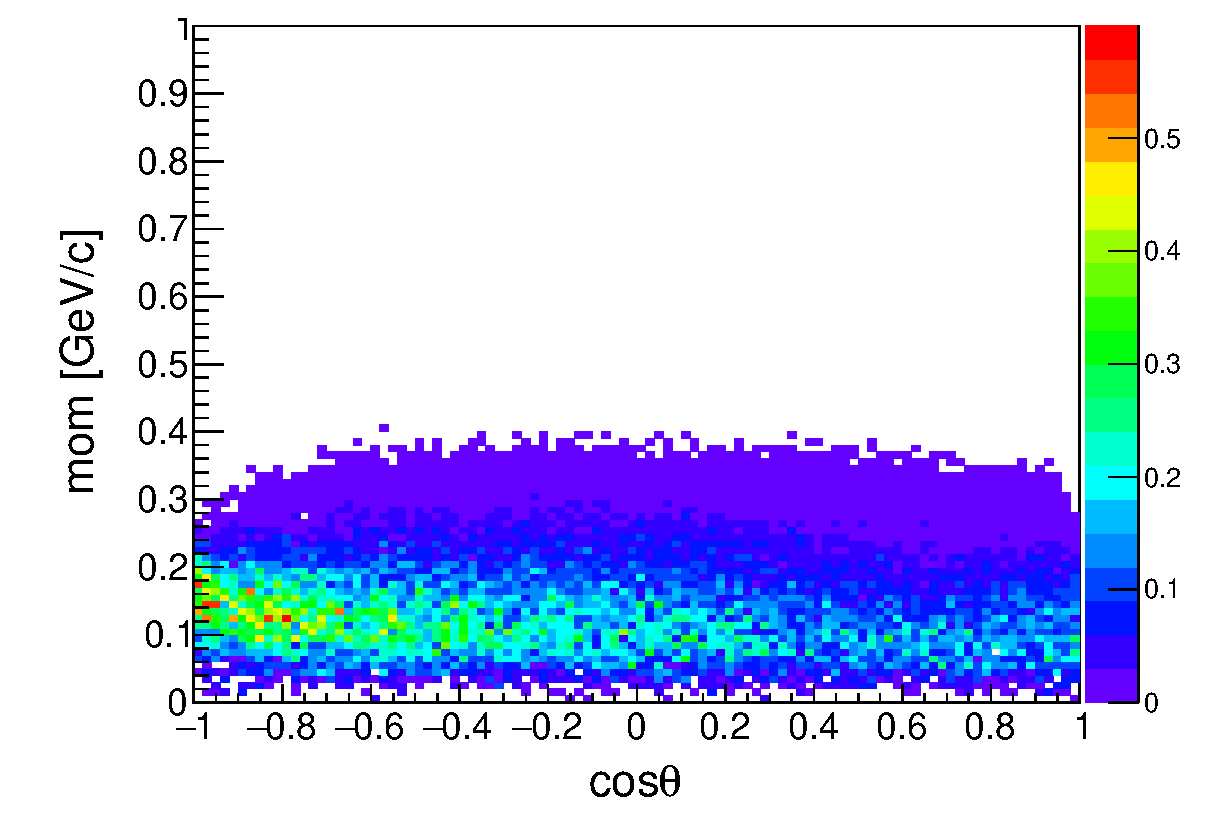
\includegraphics[width=2.7cm]{../pic/Run78/QE/K0_cos_mom_pipSm.eps}
        \end{figure} 
      }
      \tminipageTwo{
        \begin{figure}
          $K^-d \rightarrow "n"\pi^- \Sigma^+_{forward}$
          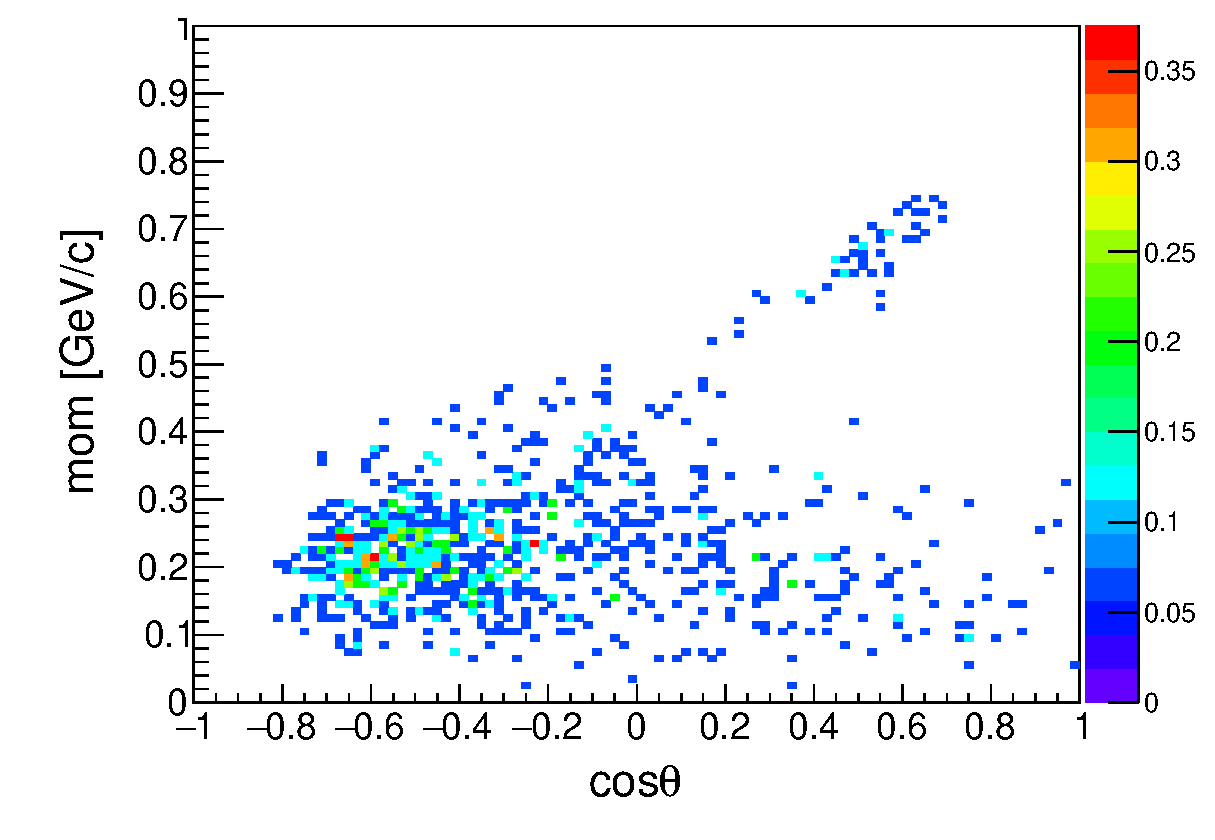
\includegraphics[width=2.7cm]{../pic/Run78/QE/K0_cos_mom_Sp.eps}
        \end{figure}
      }{
        \begin{figure}
          $K^-d \rightarrow "n"\pi^+ \Sigma^-_{forward}$
          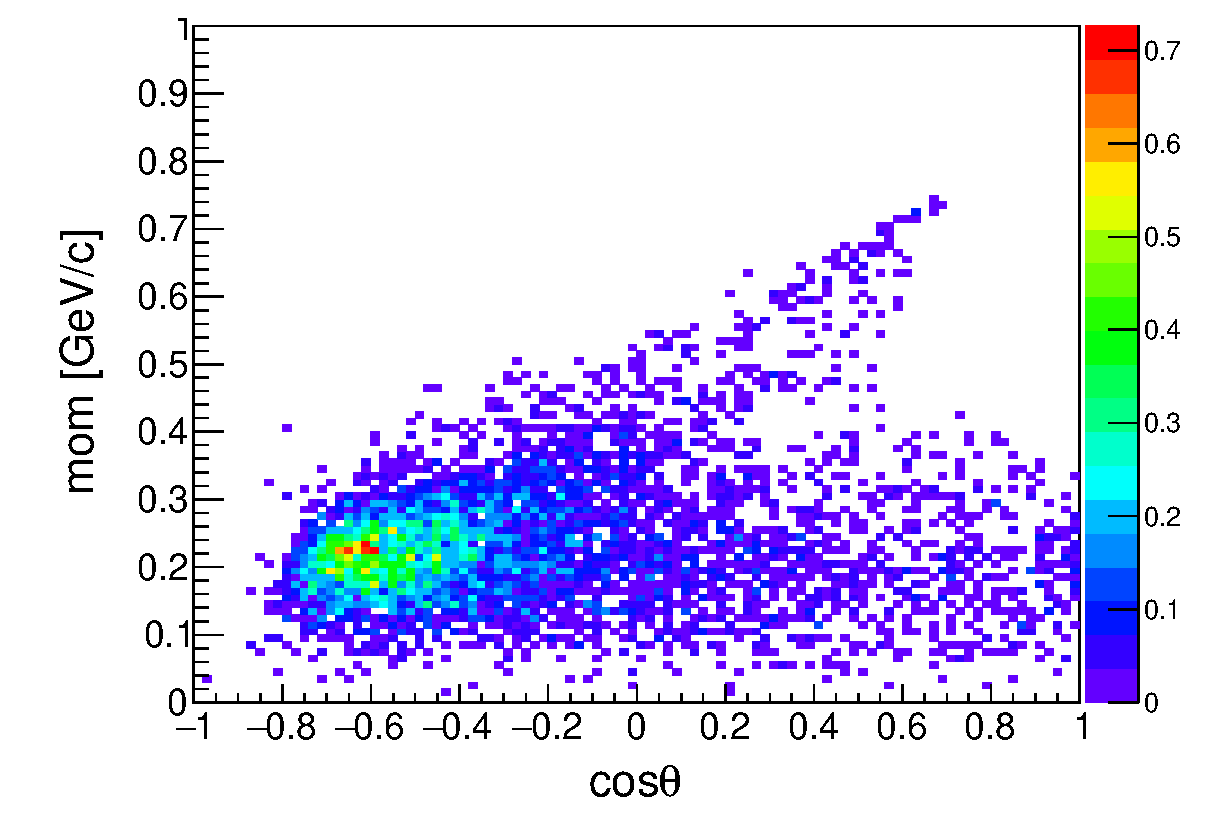
\includegraphics[width=2.7cm]{../pic/Run78/QE/K0_cos_mom_Sm.eps}
        \end{figure} 
      }
    \end{minipage}

    \begin{minipage}{0.5\hsize}
      \begin{figure}
        Background sum
        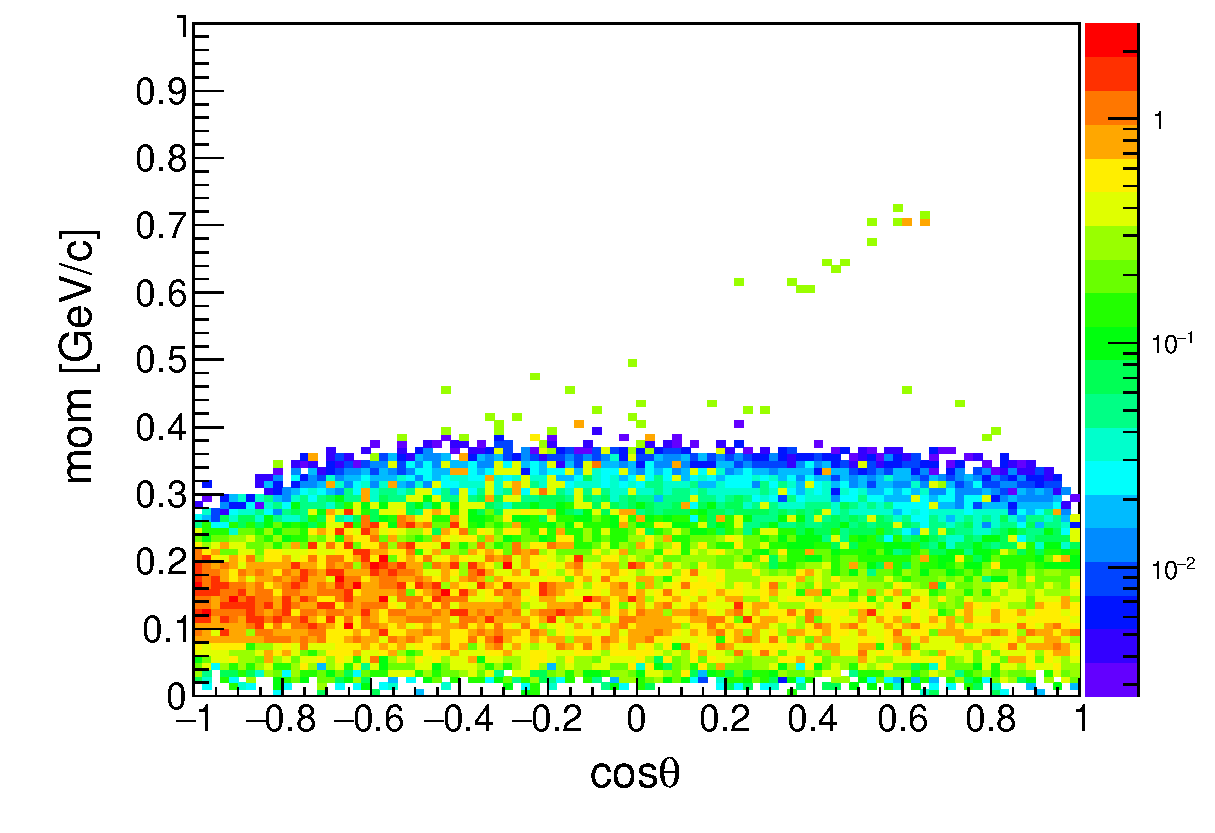
\includegraphics[width=6cm]{../pic/Run78/QE/K0_cos_mom_BG.eps}
      \end{figure}
    \end{minipage}
  \end{tabular}
  \centering
  Background spreads more wider region than data.
%  バックグラウンドはデータに比べて$\cos\theta$の広い部分に分布している。
\end{frame}

